\section{Van Kampen's Theorem}

In the spirit of computing fundamental groups (before moving on to higher notions of homotopy), we now consider how/in what way the fundamental group of a space $X$ can be understood in terms of the fundamental groups of different ``pieces'' of $X$.
\begin{boxexample}
To get an idea of the kind of result we might expect (or could hope to have), we look at a few examples:
    \begin{itemize}
    \item We know that $\pi_1(S_1)\cong \Z$, and $\pi_1(S^1\vee S^1)\cong \Z*\Z$ (the free product of $\Z$ with itself). $S^1\vee S^1$ is just two circles glued together at a point.
    \item We know that $\pi_1(S^1\times S^1)\cong \Z^2$...we can imagine $S^1\times S^1$ as $S^1\vee S^1$, with a square glued along the boundary - in other words, we can imagine filling in the boundary of $S^1\vee S^1$ with a disk $D$, visualized as a square with opposite sides identified. Now  $\pi_1(D)$ is trivial, so if we imagine that $a,b$ generate $S^1\vee S^1$ then we can see that a loop in $S^1\times S^1$ will be trivial exactly when it is in the kernel of the quotient of our square (i.e. we can see that $\pi_1(S^1\times S^1)\cong \grpres{a,b}{aba^{-1}b^{-1}} \cong \Z^2$). We can think then of $S^1\times S^1$ as a union of the disk $D$ and the quotiented boundary (isomorphic to $S^1\vee S^1$) of our disk...and to get the fundamental group, we quotient $\pi_1(S^1\vee S^1)$ by the (homotopy-class of) trivial loops in the intersection of $D\cap S^1\vee S^1$...
    \item We could also consider $S^1$ composed of ``parts'' $S^1=(S^1\setminus \{u_1\})\cup (S^1\setminus \{u_2\})$ for some distinct $u_1, u_2\in S^1$. Each of these parts $S^1\setminus \{u_i\}$ has trivial $\pi_1$, and we know that $\pi_1(S^1)\cong \Z$. \sorry
\end{itemize}
    
\end{boxexample}

The long and the short of Van Kampen's Theorem is that under the right conditions, $\pi_1$ preserves pushouts.

%we discussed an example of the klein bottle, and talked about how we can nicely understand spaces as quotients of their universal covers, which makes things nice in two dimensions and more akward but not the worst in 3 dimensions. also it was observed that all these universal covers are spaces with metrics, so each fundamental group inherits a ``maximally symmetric metric'' as a quotient of the metrics of its universal cover?

Recall that the free product is the coproduct in the category of groups. This means that if $G_{\alpha}$ and $H$ are groups, and $\varphi_{\alpha} : G_{\alpha} \to H$ are homomorphisms, then there is a unique extension $\phi : \ast_{\alpha} G_{\alpha} \to H$.

In our setup, let $X$ be a space and let $x_0 \in X$ be a basepoint. Assume there exist open, path-connected sets $A_{\alpha}$ with $x_0 \in \bigcap_{\alpha} A_{\alpha}$ and $X = \bigcup_{\alpha} A_{\alpha}$.

We know that the inclusions $A_{\alpha} \inj X$ induce maps $j_{\alpha} : \pi_1\of{A_{\alpha}; x_0} \to \pi_1\of{X; x_0}$. Since $*$ is a coproduct in $\Grp$, these are uniquely extended to a homomorphism $\phi : \ast_{\alpha} \pi_1\of{A_{\alpha}; x_0} \to \pi_1\of{X; x_0}$.

\begin{boxlemma}\label{Ch1:Lemma:VanKampen_Surjective}
    $\phi$, as defined above, is surjective provided that \sorry.
\end{boxlemma}

We can summarise everything we've done so far into one gigantic theorem. See also \cite[Chapitre 5, Théorème 1.2]{EPFLTopologie}.

\begin{boxtheorem}[Van Kampen]
    Let $X$ be a topological space with basepoint $x_0$. Assume there exist sets $A_{\alpha}$ that such that
    \begin{itemize}
        \item Each $A_{\alpha}$ is open and path-connected
        \item $x_0 \in \bigcap_{\alpha} A_{\alpha}$
        \item $A = \bigcup_{\alpha} A_{\alpha}$
        \item For all $\alpha, \beta$, $A_{\alpha} \cap A_{\beta}$ are path-connected
    \end{itemize}
    Then, the map $\phi : \ast_{\alpha} \pi_1\of{A_{\alpha}; x_0} \to \pi_1\of{X; x_0}$, obtained as a coproduct of the maps induced by the inclusions, is surjective. \newline

    If, moreover, $A_{\alpha} \cap A_{\beta} \cap A_{\gamma}$ is path-connected for all $\alpha, \beta, \gamma$, then $\pker{\phi}$ is the normal subgroup generated by $i_{\alpha \beta}(\omega) i_{\beta\alpha}(\omega)\inv$ for $\omega \in \pi_1\of{A_{\alpha} \cap A_{\beta}; x_0}$, where $i_{\alpha \beta} : \pi_1\of{A_{\alpha} \cap A_{\beta}; x_0} \to \pi_1\of{A_{\alpha}; x_0}$ is the map induced by the inclusion. \newline

    In particular,
    \begin{align*}
        \pi_1\of{X; x_0} \cong \quotient{\ast_{\alpha} \pi_1\of{A_{\alpha}; x_0}}{\pker{\phi}}
    \end{align*}
    via the first isomorphism theorem.
\end{boxtheorem}
\begin{remark}
    Before we prove this theorem, we make a few remarks.
    \begin{enumerate}
        \item Compare the statement above to the statement that if there exist $A, B \ssq X$ open such that $X = A \cup B$ and $A \cap B$ is path-connected, then $\pi_1(X) = \pi_1(A) *_{\pi_1(A \cap B)} \pi_1(B)$, ie, $\pi_1$ preserves pushouts under the right conditions \cite[Ch 5, Thm 1.2]{EPFLTopologie}. The quotient group in the version of the theorem stated in lectures is precisely the amalgamated product.\todo{Right?}

        \item Going from a 2 set version to an $n$ set version shouldn't be hugely complicated, as long as we're careful about taking quotients and amalgamated products and whatever
    \end{enumerate}
\end{remark}
For the proof, we can more or less follow \cite[Ch 5, Thm 1.2]{EPFLTopologie}.
\begin{proof}
    The only thing that we really need to check is that $\pker{\phi}$ is generated by the right elements, since we have already shown surjectivity in Lemma~\ref{Ch1:Lemma:VanKampen_Surjective}. \sorry
\end{proof}

\begin{boxexample}[The Dunce Hat]
    The \textbf{dunce hat} is the topological space obtained by making the following identifications on the (solid) triangle:
    \begin{figure}[H]
        \centering
        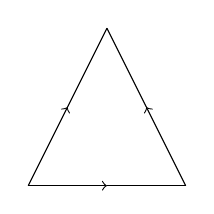
\begin{tikzpicture}
            \draw[->] (-1,0) -- (0, 0);
            \draw (0, 0) -- (1, 0);
            \draw[->] (-1,0) -- (-0.5, 1);
            \draw (-0.5, 1) -- (0, 2);
            \draw[->] (1,0) -- (0.5, 1);
            \draw (0.5, 1) -- (0, 2);
        \end{tikzpicture}
    \end{figure}
    \sorry % Split into a trapezium and a triangle or something and show, using Van Kampen, that the fundamental group is trivial
\end{boxexample}

\begin{boxcorollary}
    Given path-connected spaces $(X; x_0)$ and $(Y; y_0)$,
    \begin{align*}
        \pi_1\of{X \vee Y} \cong \pi_1\of{X; x_0} * \pi_1\of{Y; y_0}
    \end{align*}
    where we wedge them at their basepoints.
\end{boxcorollary}

\begin{boxexample}[Wedge of Projective Planes]
    Recall that $\pi_1\of{\R P^2} \cong \Zmod{2}$. Thus,
    \begin{align*}
        \pi_1\of{\R P^2 \vee \R P^2} \cong \Zmod{2} * \Zmod{2}
    \end{align*}
    This is a group where we have two generators, $a$ and $b$, and all powers of $a$ and powers of $b$ are trivial. So words look like
    \begin{align*}
        a, b, ab, ba, aba, bab, abab, baba, ababa, babab, \ldots
    \end{align*}
    We can, in fact, use this information to construct a universal cover of $\R P^2$: such a cover consists of countably many copies of $S^2$, where each is joined to the next at a pole (so it's a row of $S^2$s where the each is wedged to the next at its north pole/the other's south pole).
\end{boxexample}
